\chapter{Fundamentos teóricos} \label{chap:fundamentos-teoricos}

En este Capítulo vamos a dar una introducción varios algoritmos de aprendizaje automático.

\section{Métodos no supervisados}

Los algoritmos de aprendizaje automático no supervisados se utilizan cuando no se conoce la salida esperada. Al algoritmo de aprendizaje se le otorgan los datos de entrada y se le pide extraer información de estos datos. Las principales aplicaciones de estos algoritmos, las cuales vamos a aprovechar, son la agrupación de datos y la reducción de dimensionalidad de las variables de los mismos. Esa última es usada principalmente para poder hacer representaciones de datos multidimensionales, los cuales serian complejos de visualizar de otra forma.

La principal pega que pueden tener estos algoritmos es que, si bien no siempre son capaces de identificar conocimiento dados los datos utilizados, cuando lo obtienen, no siempre es el conocimiento que esperábamos obtener. Póngase el ejemplo de un algoritmo que tratase de agrupar rostros de personas iguales. Al no darle a priori ningún tipo de salida de ejemplo, el algoritmo puede acabar clasificando si los rostros están de frente o de lado, no precisamente lo que esperábamos. Es por ello que estos algoritmos cuentan con diversidad de parámetros para ajustarlos a nuestras necesidades, tratando de realizar la agrupación deseada.

En esta sección vamos a estudiar a fondo tres tipos de algoritmos de agrupación: el agrupamiento por k-medias, la agrupación aglomerada, y la agrupación por afinidad. Además, estudiaremos también el principal algoritmo de reducción de dimensiones, el análisis de componentes principales, PCA, de sus siglas en inglés. Los principales ejemplos y explicaciones de los algoritmos han sido inspirados por los dados en el libro \cite[Introduction to Machine Learning with Python]{machine}.

\begin{mypython}[float={h},caption={Generar datos artificiales de prueba.}]
  from sklearn.datasets import make_blobs

  X, y = make_blobs(n_samples=100, centers=4,
                  n_features=3, random_state=0)
\end{mypython}

% Artificial data
\begin{figure}[h]
  \centering
  \begin{subfigure}{0.45\textwidth}
    \centering
    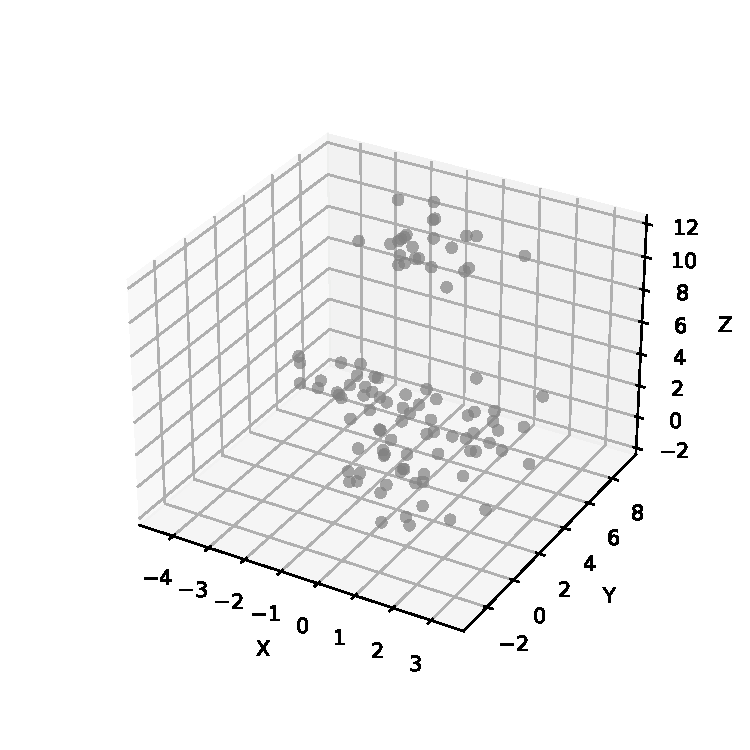
\includegraphics[width=\textwidth]{figures/artificial-data.pdf}
    \caption{}
    \label{fig:artificial-data-grey}
  \end{subfigure}
  \begin{subfigure}{0.45\textwidth}
    \centering
    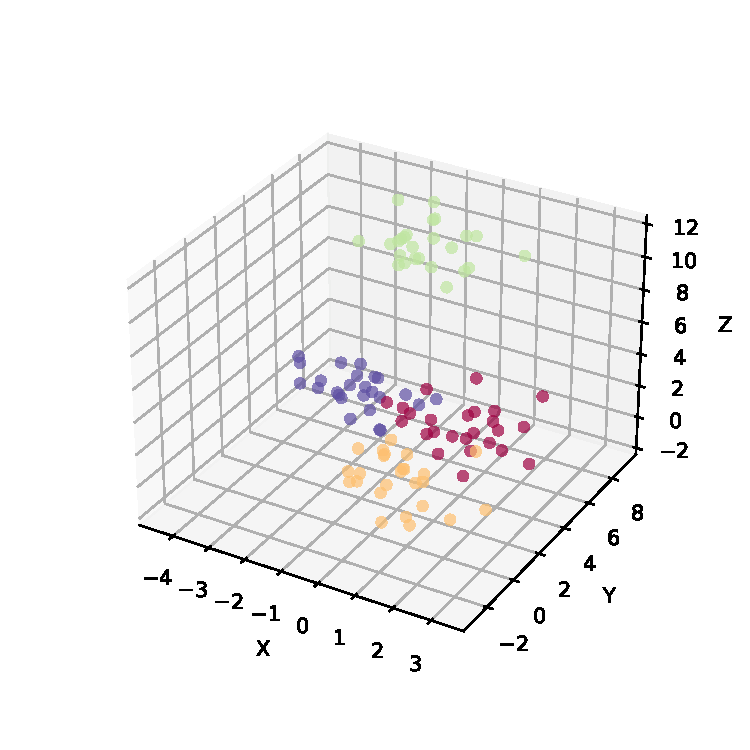
\includegraphics[width=\textwidth]{figures/artificial-data-labeled.pdf}
    \caption{}
    \label{fig:artificial-data-labeled}
  \end{subfigure}
  \caption[Datos artificiales para la prueba de algoritmos.]{Datos artificiales generados para probar algoritmos de agrupamiento. Consisten en 100 puntos tridimensionales agrupados equilibradamente al rededor de 4 centros aleatorios. \ref{fig:artificial-data-grey} En gris los puntos generados sin asignar ninguna etiqueta. Estos serán los datos que recibirán los algoritmos para procesar y agrupar. \ref{fig:artificial-data-labeled} Datos etiquetados según el grupo al que pertenecen. Esto nos ayudará a verificar la eficacia de nuestros algoritmos.}

  \label{fig:artificial-data}
\end{figure}

En la tabla \ref{tab:colab-links} está el enlace para poder ejecutar el código en el \textit{backend} de Google.

\newpage
\subsection{Análisis de componentes principales}
(EXPLICACIÓN PCA)

\begin{mypython}[float={h},caption={Escalar y estandarizar los datos.}]
  from sklearn.preprocessing import StandardScaler

  scaler = StandardScaler()
  scaler.fit(X)
  features_scaled = scaler.transform(X)
\end{mypython}

\begin{mypython}[float={h},caption={Realizar un PCA.}]
  from sklearn.preprocessing import StandardScaler

  pca = PCA(n_components=3)
  pca.fit(features_scaled)
  X_reduced = pca.transform(X)
\end{mypython}
% PCA
\begin{figure}[]
  \centering
  \begin{subfigure}{\textwidth}
    \centering
    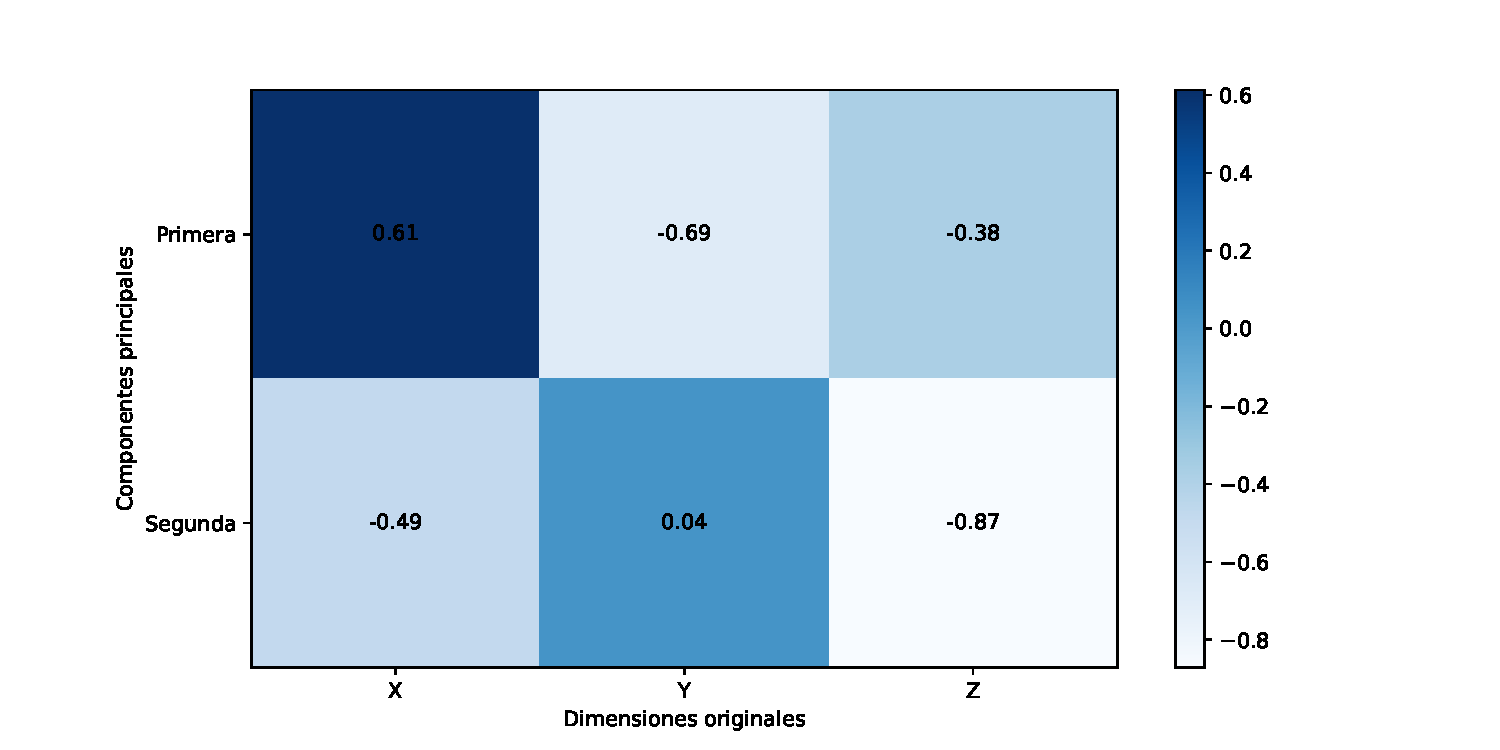
\includegraphics[width=\textwidth]{figures/pca-color-ponderation.pdf}
    \caption{}
    \label{fig:pca-color-ponderation}
  \end{subfigure}
  \begin{subfigure}{0.45\textwidth}
    \centering
    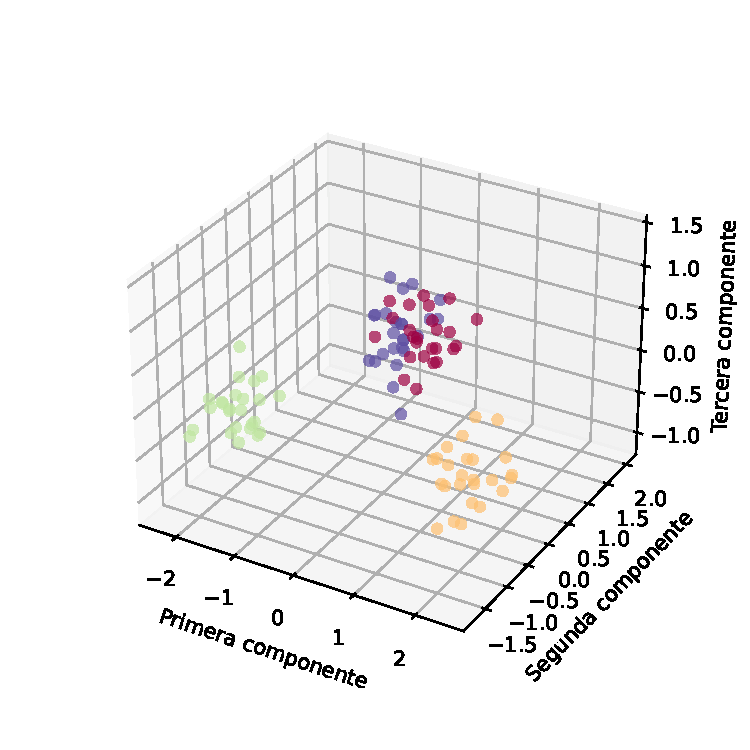
\includegraphics[width=\textwidth]{figures/pca-3d-labeled.pdf}
    \caption{}
    \label{fig:pca-3d-labeled}
  \end{subfigure}
  \begin{subfigure}{0.45\textwidth}
    \centering
    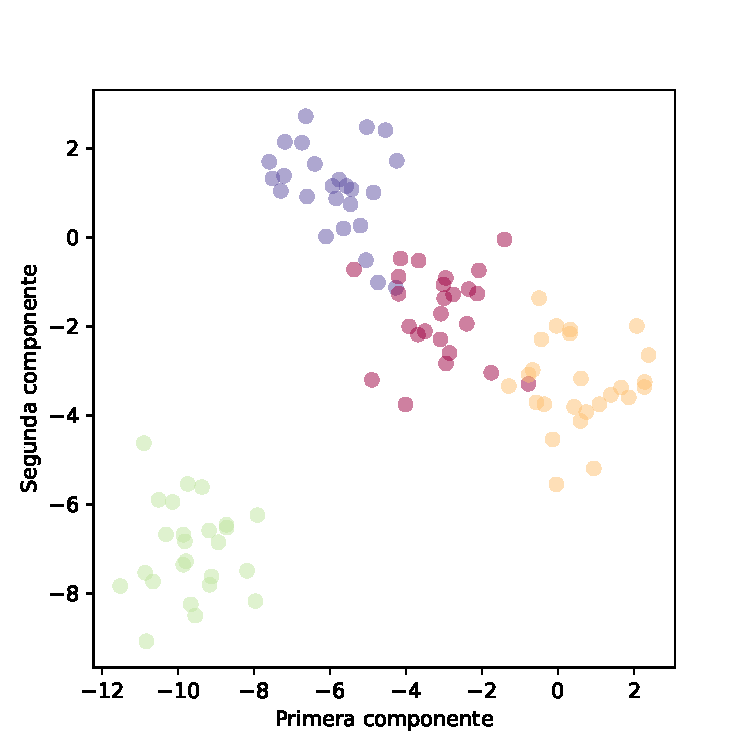
\includegraphics[width=\textwidth]{figures/pca-labeled.pdf}
    \caption{}
    \label{fig:pca-labeled}
  \end{subfigure}
  \caption[Probando un PCA.]{\ref{fig:pca-color-ponderation} Mapa de calor con las ponderaciones asignadas por el PCA a cada uno de las dimensiones originales. \ref{fig:pca-3d-labeled} Visualización de los datos previamente generados tras escalarlos y aplicarles la PCA. Los colores de los grupos se mantienen, pero los ejes ahora representan las componentes principales, en vez de las dimensiones originales. \ref{fig:pca-labeled} Visualización de las dos primeras componentes principales sobre el plano. Este será el formato en el que visualizaremos más adelante las agrupaciones ejercidas sobre datos reales de dimensionalidad alta.}
  \label{fig:pca}
\end{figure}

\newpage
\subsection{Agrupamiento por K-medias}

El algoritmo de k-medias clasifica los datos separando los datos en $n$ grupos de con la misma varianza.

El algoritmo comienza inicializando aleatoriamente $n$ centroides, siendo $n$ el número de agrupaciones que se le han dicho que realice. Estos centroides serán los centros de las agrupaciones que va a realizar, no tienen por qué pertenecer a los datos, pero sí que están contenidos en su misma dimensión. En cada iteración, el algoritmo asigna a cada punto de los datos el centroide más próximo y luego asigna a cada agrupación un nuevo centroide calculado como la media de los datos que se han asignado a dicha agrupación.

Formalmente, el algoritmo divide un conjunto de $n$ puntos $x$ en $k$ agrupaciones disjuntas $C$, cada una descrita por la media $\mu_j$ de los puntos en la agrupación. Para ello, el algoritmo trata de encontrar los centroides que minimicen

\begin{equation}
  \sum\limits_{i=0}^n \underset{\mu_j \in C}{\operatorname{min}} (|| x_i - \mu_j||^2)
\end{equation}

El algoritmo finaliza cuando una iteración no realice ninguna modificación de las agrupaciones.

\newpage
\begin{mypython}[float={h},caption={k-medias.}]
  from sklearn.cluster import KMeans

  kmeans = KMeans(n_clusters=2, n_init="auto"
  kmeans_assigment = kmeans.fit_predict(X)
\end{mypython}

% k-means
\begin{figure}[h]
  \centering
  \begin{subfigure}{0.45\textwidth}
    \centering
    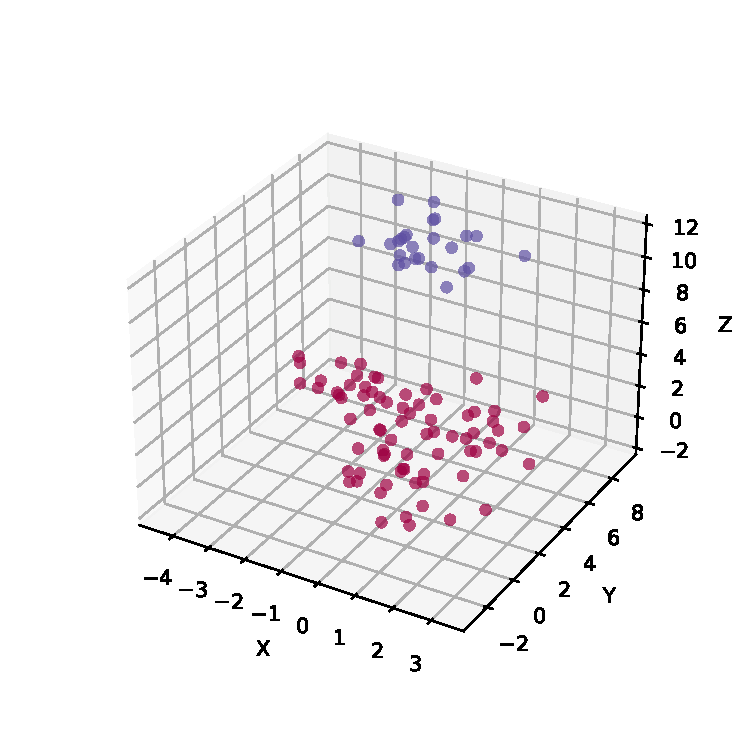
\includegraphics[width=\textwidth]{figures/kmeans-3d.pdf}
    \caption{}
    \label{fig:kmeans-3d}
  \end{subfigure}
  \begin{subfigure}{0.45\textwidth}
    \centering
    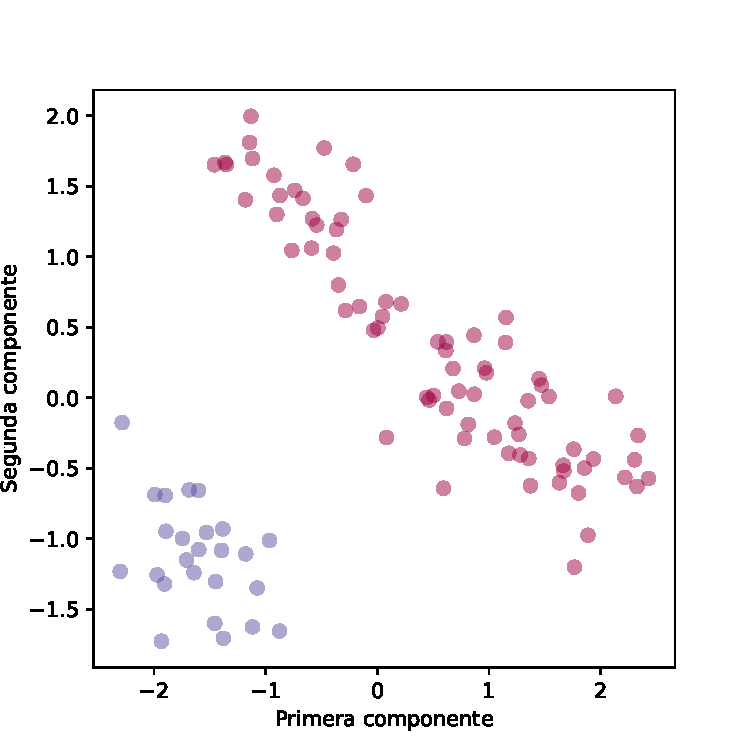
\includegraphics[width=\textwidth]{figures/kmeans-pca.pdf}
    \caption{}
    \label{fig:kmeans-pca}
  \end{subfigure}
  \caption[Prueba del algoritmo de k-medias.]{\ref{fig:kmeans-3d} Visualización sobre los datos sin modificar de los grupos que ha realizado el algoritmo de k-medias. \ref{fig:kmeans-pca} Visualización de los grupos realizados sobre los datos procesados por el PCA.}
  \label{fig:kmeans}
\end{figure}

\newpage
\subsection{Agrupación aglomerada}
(EXPLICACIÓN ALGORITMO)

\begin{mypython}[float={h},caption={Agrupación aglomerada.}]
  from sklearn.cluster import AgglomerativeClustering

  agg = AgglomerativeClustering()
  agg_assigment = agg.fit_predict(X)
\end{mypython}

% Agglomerative
\begin{figure}[h]
  \centering
  \begin{subfigure}{0.45\textwidth}
    \centering
    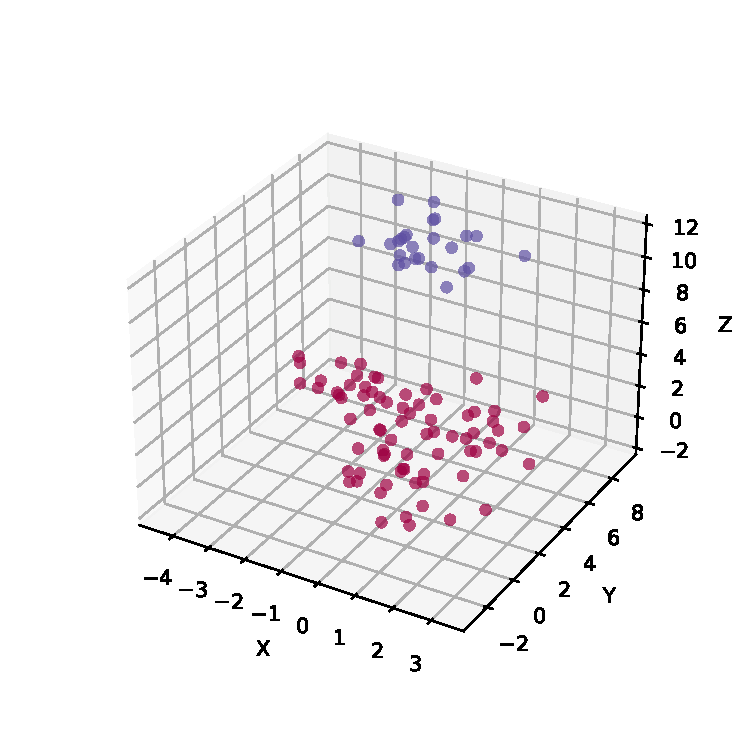
\includegraphics[width=\textwidth]{figures/agglomerative-3d.pdf}
    \caption{}
    \label{fig:}
  \end{subfigure}
  \begin{subfigure}{0.45\textwidth}
    \centering
    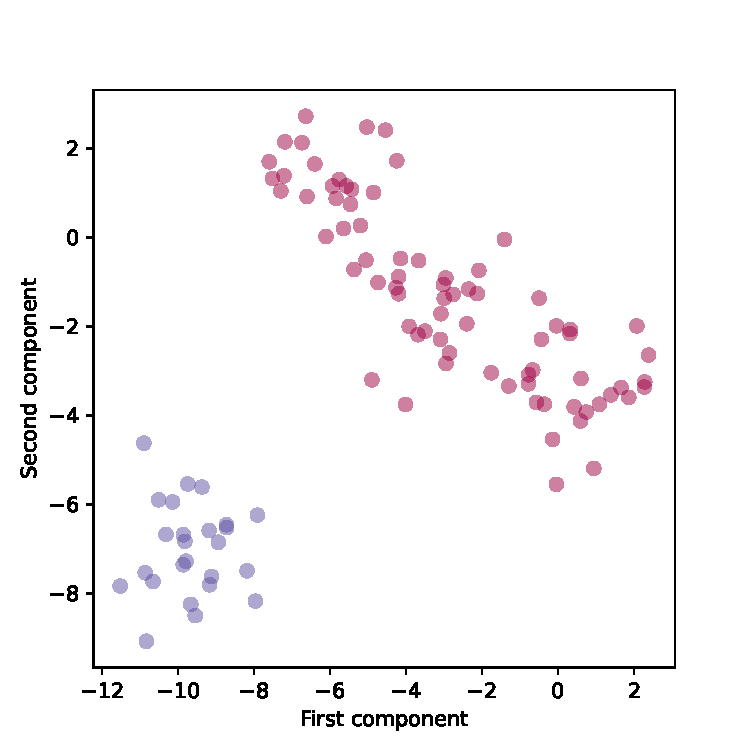
\includegraphics[width=\textwidth]{figures/aglomerative-pca.pdf}
    \caption{}
    \label{fig:}
  \end{subfigure}
  \caption[Prueba del algoritmo aglomerativo.]{(EXPLICACIÓN FIGURA)}
  \label{fig:}
\end{figure}

\newpage
\subsection{Agrupación por afinidad}

El algoritmo de propagación de afinidad crea agrupaciones mandando mensajes entre pares de puntos hasta que converge. La principal cualidad de este algoritmo es que, a diferencia con la mayoría de algoritmos de agrupamiento, no necesita saber el número de agrupaciones a realizar de antemano, sino que las genera dinámicamente.

(TERMINAR EXPLICACIÓN ALGORITMO)

\begin{mypython}[float={h},caption={Propagación de afinidad.}]
  from sklearn.cluster import AffinityPropagation

  aff = AffinityPropagation()
  aff_assigment = aff.fit_predict(X)
\end{mypython}

% Agglomerative
\begin{figure}[h]
  \centering
  \begin{subfigure}{0.45\textwidth}
    \centering
    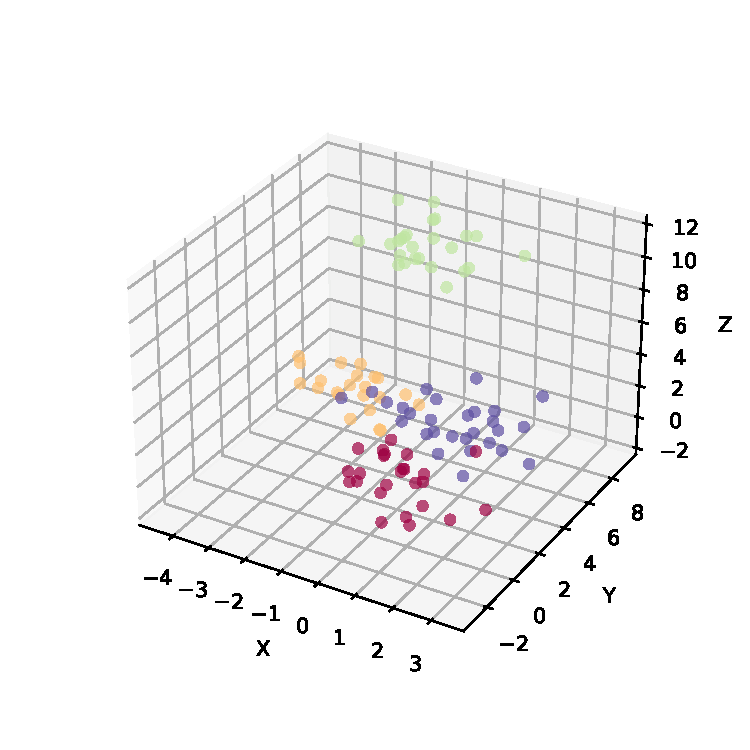
\includegraphics[width=\textwidth]{figures/affinity-3d.pdf}
    \caption{}
    \label{fig:}
  \end{subfigure}
  \begin{subfigure}{0.45\textwidth}
    \centering
    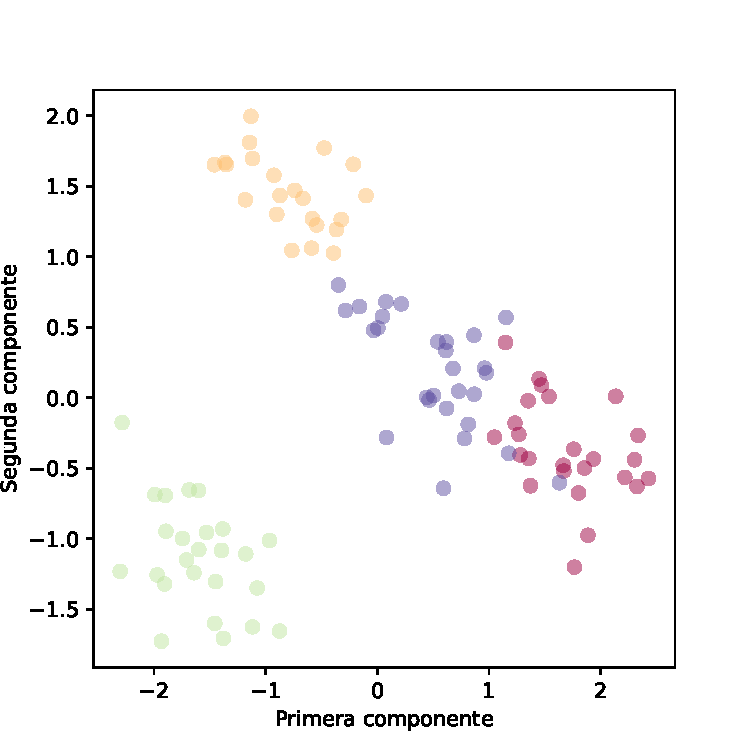
\includegraphics[width=\textwidth]{figures/affinity-pca.pdf}
    \caption{}
    \label{fig:}
  \end{subfigure}
  \caption[Prueba del algoritmo de propagación de afinidad.]{(EXPLICACIÓN FIGURA)}
  \label{fig:}
\end{figure}

\newpage
\section{Métodos supervisados}
(POR HACER)

\cite[Deep Learning with PyTorch]{pytorch}
\subsection{Red neuronal}